\documentclass[a4paper,10pt]{article}
\usepackage[vcentering,dvips]{geometry}

\newcommand{\linux}{\mbox{\sc LINUX}}
\newcommand{\awk}{\mbox{\sc awk}}
\newcommand{\sort}{\mbox{\sc sort}}

\newcommand {\articleTitle}{Informe Trabajo Pr\'actico 1}

% misc
\newcommand {\murl}[2]{\href{#1}{#2}}

% marcas / nombres de cosas usadas 
\usepackage[spanish]{babel}
\usepackage{graphicx}
\usepackage{graphics}
\usepackage[utf8]{inputenc}
\usepackage{subfigure}
\usepackage[pdftitle=\articleTitle
	pdfauthor={},
	pdfsubject={},
	pdfkeywords={} 
]{hyperref}

\usepackage{verbatim}
\usepackage{rotating}
% inclusion de codigo fuentes
\usepackage{listings}
\lstloadlanguages{c}

\author
{
	Pablo Giorgi,
	Santiago Perez De Rosso,
	Luciano Zemin
}

\date{Abril 2011}
% Title
\title{\articleTitle}

\begin{document}
\bibliographystyle{acm}
\maketitle

\tableofcontents

\section{Introducción}

En el presente informe se presenta las soluciones correspondientes al descifrado
de los archivos provistos por la c\'atedra y el an\'alisis de las cuestiones
planteadas en el punto 4 del Trabajo Pr\'actico 1.

\section{Descifrado de los archivos provistos por la c\'atedra}

Se desencriptaron los 6 archivos provistos por la c\'atedra
\emph{fun6AESCBC.wav}, \emph{fun6AESCFB.wav}, \emph{fun6AESOFB.wav},
\emph{fun6DESCBC.wav}, \emph{fun6DESOFB.wav} utilizando la clave \emph{sorpresa}
con el algoritmo y modo indicado en el nombre del archivo. Se obtuvo
el mismo fragmento de la canción \emph{El matador} de los \emph{Fabulosos Cadillacs}
en todos los casos.

\section{An\'alisis de las cuestiones planteadas en el punto 4 del Trabajo Pr\'actico 1}

Para analizar el primer punto se toma el archivo \emph{fa-do.wav}

....

Respecto al punto 4.8 se encripta el archivo \emph{fa-do.wav} utilizando DES OFB.
Se cambia un bit del texto cifrado (en el byte 4673) y se desencripta. Al comparar
el archivo original con el desencriptado corriendo
\begin{lstlisting}
cmp -l results/48/fa-do.wav results/48/fa-doDesencriptado.wav 
\end{lstlisting}
se obtiene 
\begin{lstlisting}
 4673 121 120
\end{lstlisting}
Esto indica que en el byte 4673 hay una diferencia de un bit.
\begin{figure}
	\begin{center}
		\subfigure{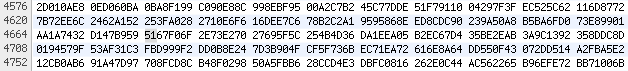
\includegraphics[scale=0.6]{../results/48/fa-do.png}}
		\subfigure{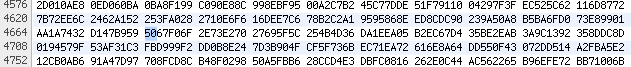
\includegraphics[scale=0.6]{../results/48/fa-doModificado.png}}
	\end{center}
	\caption{Visualización del archivo original \emph{fa-da.wav} y del archivo obtenido 
		al desencriptar el cifrado modificado con la diferencia marcada.}
	\label{fig:48}
\end{figure}
Esto se condice con la teor\'ia ya que una de las caracter\'isticas de OFB es que si
hay uno o m\'as bits con errores en cualquier caracter $ c_{j} $ del texto cifrado
esto solo afecta el descifrado de solo ese caracter. Y dado el texto plano se van a ver
los bits complementados respecto al original sin error en las mismas posiciones donde 
se cambiaron los bits del texto cifrado. En la figura \ref{fig:48} se muestra una 
parte del archivo original \emph{fa-do.wav} y el archivo obtenido al desencriptar
el cifrado alterado.

Finalmente, respecto al punto 4.9 se utiliza DES con el m\'etodo ECB para encriptar
los archivos \emph{do-fa.wav} y \emph{si-mi.wav} con el objetivo de comparar la salida
con el archivo \emph{incogDES.wav} y as\'i determinar que notas tiene el archivo
\emph{incogDES.wav}. Analizando los resultados con el Audacity se puede ver en la figura
\ref{fig:DESAudacityCmp} como la onda correspondiente al archivo \emph{si-mi.wav} encriptado
es igual a la correspondiente al archivo \emph{incogDES.wav} para la primera parte y luego 
la onda correspondiente al archivo \emph{do-fa.wav} encriptado
es igual a la correspondiente al archivo \emph{incogDES.wav} para la ultima parte . De esta forma,
sin desencriptar
el archivo \emph{incogDES.wav} se puede decir que \'este posee las notas \emph{si} y \emph{fa}.
Desencriptando el archivo se verifica empíricamente esto supuesto.
\begin{figure}
	\begin{center}
		\subfigure{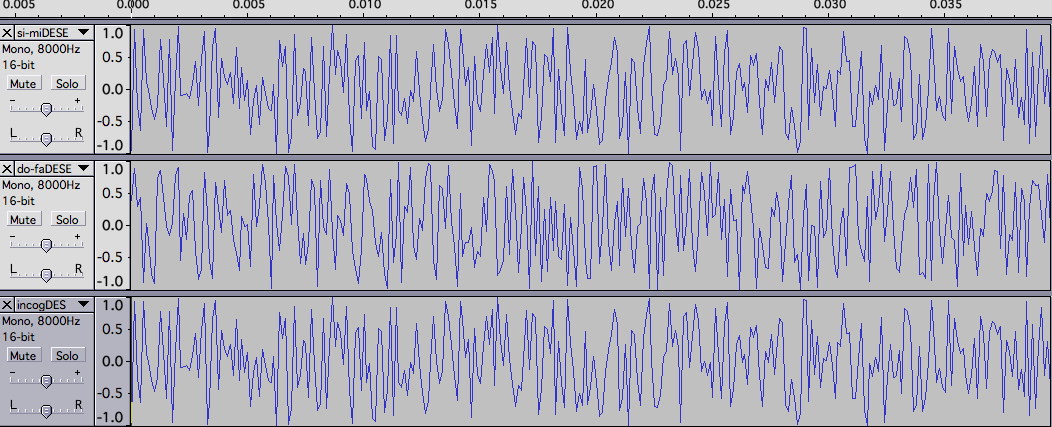
\includegraphics[scale=0.4]{../results/49/DES/audacityCmp1.png}}
		\subfigure{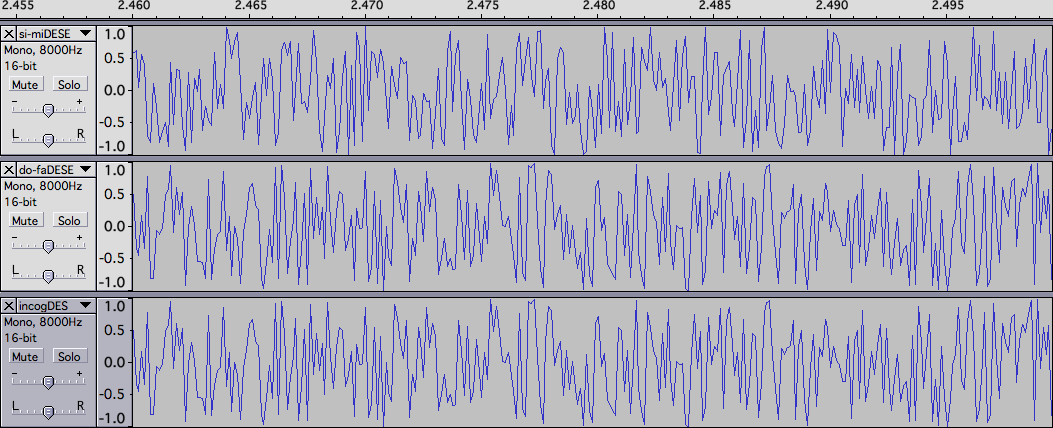
\includegraphics[scale=0.4]{../results/49/DES/audacityCmp2.png}}
	\end{center}
	\caption{Visualización de los archivos \emph{si-miDESECB.wav}, \emph{do-faDESECB.wav} y
		\emph{incogDES.wav} en el Audacity.}
	\label{fig:DESAudacityCmp}
\end{figure}

Lo mismo se realiza para el caso donde se debe utilizar AES con el m\'etodo ECB para encriptar
los archivos \emph{fa-do.wav} y \emph{mi-si.wav} con el objetivo de comparar la salida
con el archivo \emph{incogAES.wav} y as\'i determinar que notas tiene el archivo
\emph{incogAES.wav}. Sin desencriptar el archivo \emph{incogAES.wav} se puede decir que \'este
posee las notas \emph{fa} y \emph{si}. En la figura \ref{fig:AESAudacityCmp} se ve las ondas
pertinentes con el Audacity. Desencriptando el archivo se verifica empíricamente esto supuesto.
\begin{figure}
	\begin{center}
		\subfigure{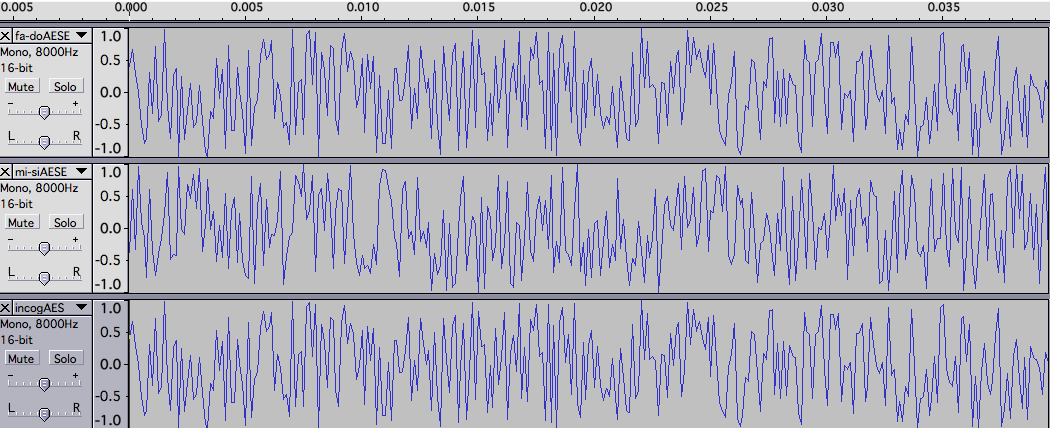
\includegraphics[scale=0.4]{../results/49/AES/audacityCmp1.png}}
		\subfigure{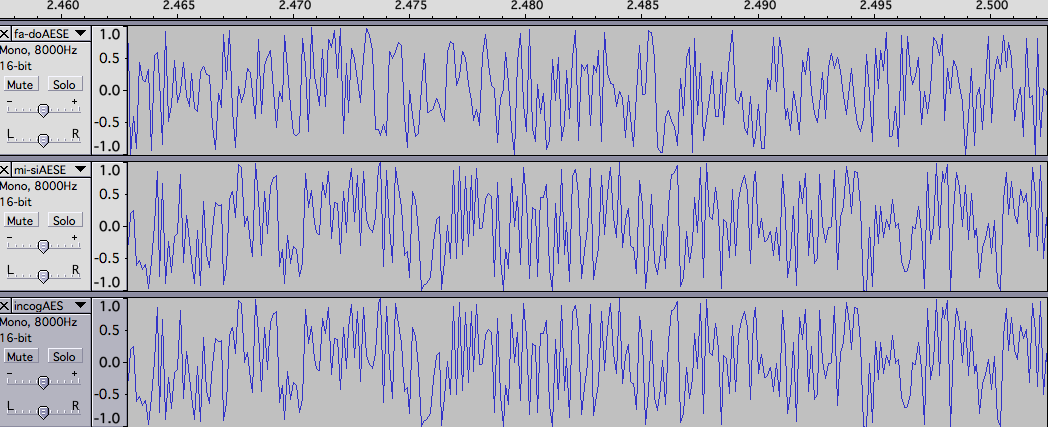
\includegraphics[scale=0.4]{../results/49/AES/audacityCmp2.png}}
	\end{center}
	\caption{Visualización de los archivos \emph{fa-daAESECB.wav}, \emph{mi-siAESECB.wav} y
		\emph{incogAES.wav} en el Audacity.}
	\label{fig:AESAudacityCmp}
\end{figure}
\end{document}
